\begin{figure}[t]
\uwsinglespace
\begin{center}
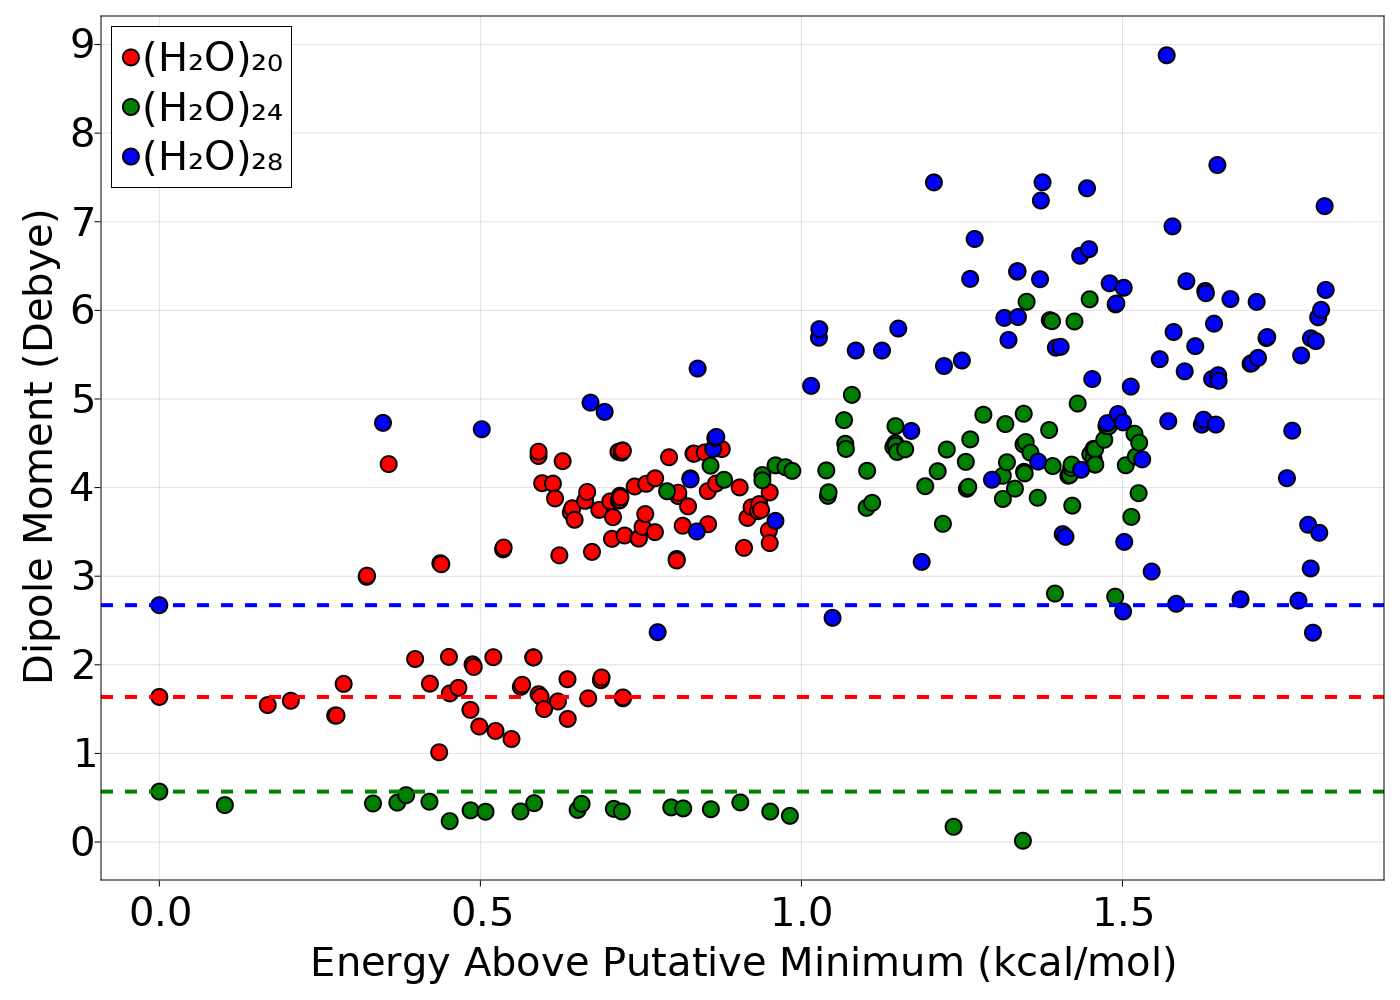
\includegraphics[width=.85\textwidth]{Figures/Chapter_6/all_clathrate_cages_dipole_vs_energy.png}
\end{center}
\begin{spacing}{1.0}
\caption[Comparison of the dipole moment of the 100 lowest energy structures of \ce{(H2O)_{20}}, \ce{(H2O)_{24}}, and \ce{(H2O)_{28}} to the energy of each configuration. The binding energies are shown as the energy difference between each structure and the lowest energy cage of that size. All data in this figure come from the TTM2.1-F potential. Dashed lines show the dipole moment of the putative minimum structure, which always corresponds to one of the lowest energy configurations.]{Comparison of the dipole moment of the 100 lowest energy structures of \ce{(H2O)_{20}}, \ce{(H2O)_{24}}, and \ce{(H2O)_{28}} to the energy of each configuration. The binding energies are shown as the energy difference between each structure and the lowest energy cage of that size. All data in this figure come from the TTM2.1-F potential. Dashed lines show the dipole moment of the putative minimum structure, which always corresponds to one of the lowest energy configurations.}\label{fig:MBE_III_F8}
\end{spacing}
\end{figure}